\subsection{Tiefensuche}
Um dem Spieler einen möglichst optimalen Stoss vorzuschlagen, sollte nicht nur der aktuelle Spielstand,
sondern auch die zukünftigen Spielstände und deren mögliche Stösse berücksichtigt werden.
Ein Stoss ist nur gut, wenn er für die Darauffolgenden eine ebenso gute, wenn nicht bessere, Ausgangslage bietet.
Ein guter Stoss in der aktuellen Situation kann evtl. zu schwierigeren Stössen führen, weil der Spielball schlecht platziert wurde.
Daher wurde beim Lösungsdesign des Suchalgorithmus darauf geachtet, dass eine Suche über mehrere Stösse ermöglicht wird.
Es handelt sich immer noch um eine Graphensuche, deren Suchraum jedoch erweitert wird.
Ein korrespondierender Suchbaum wird in Abbildung \ref{fig:suchbaum_tiefensuche} veranschaulicht.
Die orangenen Knoten bilden die Root-Knoten, die Repräsentation der Ziellöcher. Die grünen Knoten sind
Expansionsknoten. Diese stehen z.B. für einen Weg über eine Kugel oder eine Bande. Die beiden Knoten sind bereits aus
Kapitel \ref{sec:kandidatensuche} bekannt. Sobald die weisse Kugel expandiert wird, ist eine Kandidatensuche beendet und
es startet eine Simulation. Die Simulation wird beim Durchführen des Suchalgorithmus ebenfalls als Knoten in diesem
Suchbaum angesehen, hier blau eingefärbt. Nach der Berechnung eines Simulationsknotens kann die Suche bei genügender
Tiefe beendet oder wie in Ebene 3 fortgeführt werden. Das Resultat des Simulationsknotens bildet den neuen Spielstand
und es werden neue Root-Knoten darauf basierend expandiert. Die Suche kann so zukünftige Stösse in die Bewertung
des aktuellen Stosses einbeziehen.
Das Resultat der Tiefensuche sind nicht mehr nur einzelne Stösse, sondern Abfolgen von Stössen, welche nacheinander
ausgeführt werden könnten.

\begin{figure}[h!]
    \begin{center}
        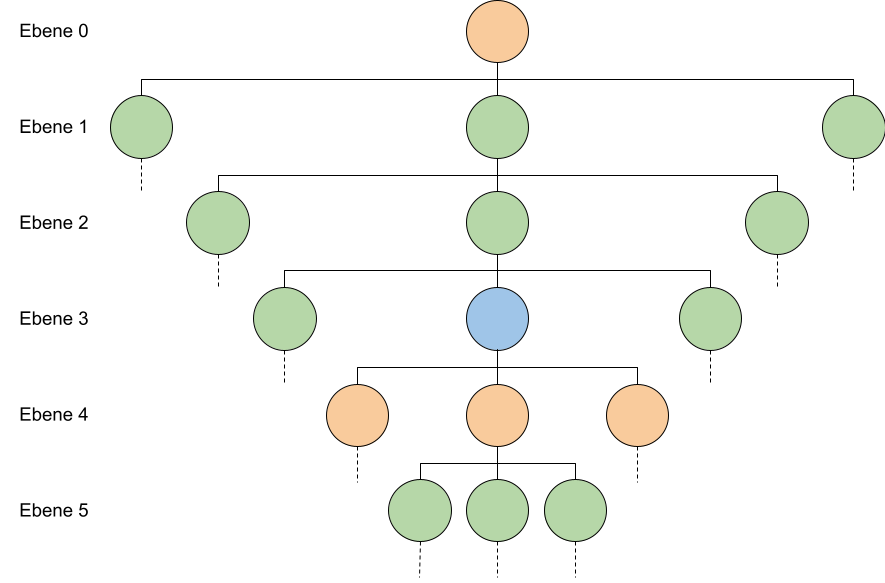
\includegraphics[width=0.7\linewidth]{../common/03_billiard_ai/resources/38_tiefensuche_suchbaum.png}
    \end{center}
    \caption{Suchbaum der Tiefensuche}
    \label{fig:suchbaum_tiefensuche}
\end{figure}

\subsubsection{Regeln für Snooker}\label{kap:tiefensuche:regeln_fuer_snooker}
Wird über mehrere Stösse gesucht, sind gewisse Regeln des Spiels einzuhalten. Bei Snooker werden abwechslungsweise rote
und farbige Kugeln versenkt, solange noch rote Kugeln auf dem Tisch sind. Die farbigen Kugeln haben unterschiedliche
Werte: Gelb(2), Grün(3), Braun(4), Blau(5), Pink(6), Schwarz(7)\cite{stoppball:spielregel:snooker}.\\
Gibt es noch eine oder mehrere rote Kugeln zu spielen, wird die versenkte farbige Kugel, ausser die Rote, wieder
auf ihrem Spot (Aufsetzmarke) platziert. Ist der Spot nicht frei, so wird sie auf den nächsthöherwertigen Spot gelegt. Die Wertung
der Spots entspricht der Wertung der Kugeln, welche bei der Ausgangsstellung platziert wurden. Die Ausgangsstellung ist in
Abbildung \ref{fig:snooker_ausgangslage} veranschaulicht. Wenn alle Spots belegt sind, wird die Kugel so nah wie möglich an ihrem ursprünglichen
Spot in Richtung der Kopfbande\footnote{Die Kopfbande ist diejenige, welcher der schwarzen Kugel bei der Ausgangsstellung am
nächsten ist.} platziert\cite{stoppball:spielregel:snooker}.

\begin{figure}[h!]
    \begin{center}
        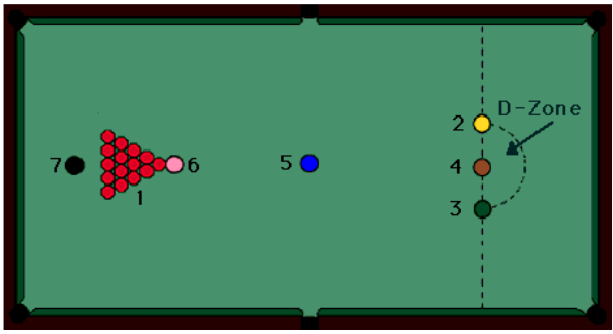
\includegraphics[width=0.4\linewidth]{../common/03_billiard_ai/resources/39_snooker_ausgangslage.png}
    \end{center}
    \caption{Ausgangslage bei Snooker\cite{stoppball:spielregel:snooker}}
    \label{fig:snooker_ausgangslage}
\end{figure}

Diese möglichst nahe Platzierung wurde über eine Suche nahe dem Spot in einem diskretisierten Raum implementiert.
Abbildung \ref{fig:snooker_spot_replacement} veranschaulicht eine solche Situation, in der die Position $s$ besetzt
ist und daher eine möglichst nahe Platzierung erforderlich ist.
Es wird angenommen, dass sich die Kopfbande auf der rechten Seite befindet. Demnach wird zuerst eine Position in dieser
Richtung geprüft, danach eine Position in senkrechter Richtung zur Kopfbande und anschliessend die Position entgegengesetzt
zur Kopfbande.
Dies ist in Abbildung \ref{fig:snooker_spot_replacement} in den Schritten $1a$ bis $1d$ zu sehen.
Die Fringe $f$ beinhaltet potenzielle Positionen für die zu platzierende Kugel, die noch auf Verfügbarkeit geprüft werden müssen.
Zu Beginn enthält $f$ nur die belegte Position $s$.
Ist eine Platzierung nicht möglich, werden die Positionen $a_1$ bis $a_4$ als neue Fringe betrachtet. Danach werden die Positionen
innerhalb der Fringe wiederum zuerst Richtung Kopfbande, danach in senkrechter Richtung zu dieser und anschliessend noch entgegengesetzt
auf Verfügbarkeit geprüft. Zu sehen in den Schritten $2a$ bis $2d$. Dies wird fortgeführt, solange die Kugel nicht platziert
werden konnte und die möglichen Positionen nicht zu weit vom Spot entfernt sind oder ausserhalb des Tisches liegen.
Wenn die Kugel nicht platziert werden konnte, wird dies als Fehler betrachtet und die Suche wird abgebrochen.

\begin{figure}[h!]
    \begin{center}
        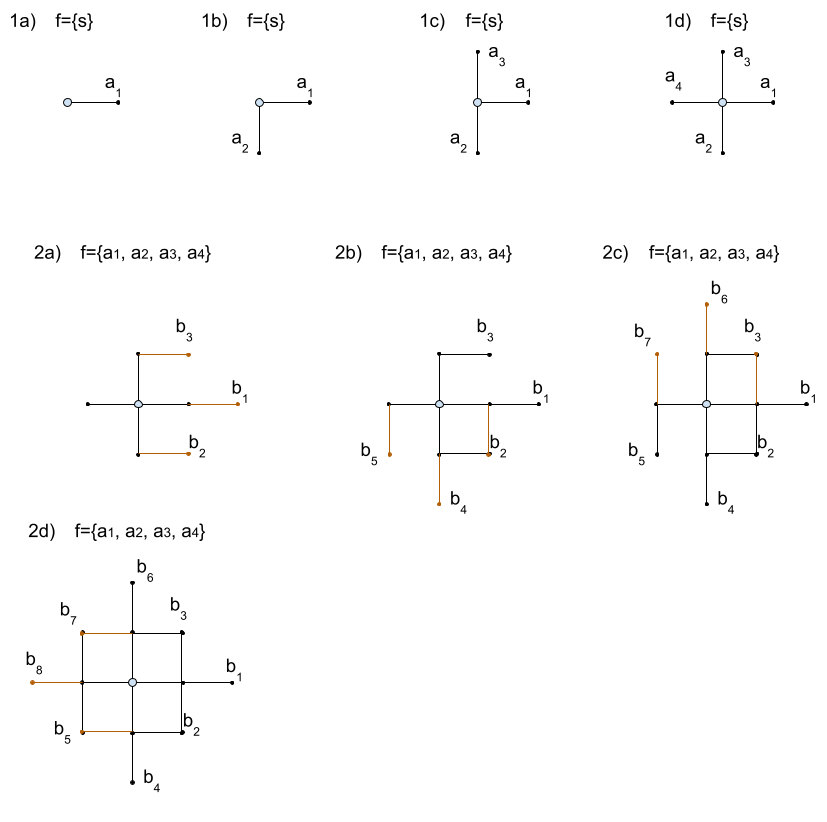
\includegraphics[width=0.6\linewidth]{../common/03_billiard_ai/resources/40_replatzierung_kugel.png}
    \end{center}
    \caption{Replatzierung einer Kugel nahe am Spot $s$}
    \label{fig:snooker_spot_replacement}
\end{figure}

Gibt es keine roten Kugeln mehr, werden die farbigen Kugeln in der Reihenfolge ihrer Punkte aufsteigend,
also Gelb, Grün, Braun, Blau, Pink, Schwarz versenkt und das Spiel ist beendet\cite{stoppball:spielregel:snooker}.
